\documentclass[addpoints,12pt, answers]{exam}

\usepackage{amsmath, amsthm, amssymb, amsfonts}
\usepackage{thmtools}
\usepackage{graphicx}
\usepackage[hidelinks]{hyperref}
\usepackage[utf8]{inputenc}
\usepackage[english]{babel}
\usepackage{framed}
\usepackage[dvipsnames]{xcolor}
\usepackage{tcolorbox}
\usepackage{tabto}
\usepackage{titling}
\usepackage{tikz}
\usepackage{dirtree}

\usetikzlibrary{patterns}
\tikzset{
level distance=13mm,
every child/.style={line width=0.3mm},
black/.style={text=white, circle, draw=black, line width=0.4mm, inner sep=4pt},
red/.style={text=white, circle, draw=black, line width=0.4mm, inner sep=4pt},
unknown/.style={text=white, circle, draw=black, line width=0.4mm, inner sep=4pt, preaction={fill, pink!90!black}, pattern=north east lines,distance=0.5pt},
}

\usepackage{changepage} % for the adjustwidth environment


\colorlet{LightGray}{White!90!Periwinkle}
\colorlet{LightOrange}{Orange!15}
\colorlet{LightGreen}{Green!15}

\newcommand{\HRule}[1]{\rule{\linewidth}{#1}}

\declaretheoremstyle[name=Theorem,]{thmsty}
\declaretheorem[style=thmsty,numberwithin=section]{theorem}
\tcolorboxenvironment{theorem}{colback=LightGray}

\declaretheoremstyle[name=Proposition,]{prosty}
\declaretheorem[style=prosty,numberlike=theorem]{proposition}
\tcolorboxenvironment{proposition}{colback=LightOrange}

\declaretheoremstyle[name=Principle,]{prcpsty}
\declaretheorem[style=prcpsty,numberlike=theorem]{principle}
\tcolorboxenvironment{principle}{colback=LightGreen}

%% This latex package provides all the utilities for
%% 15150 assignments development.
%% This package is intended to be included in writeup.tex at
%% problem level.
%% For a full list of custom commands, check 15150toolbox.md
%%
%% @author: Jolin Zhou
%% @email: jiulingz@andrew.cmu.edu

\NeedsTeXFormat{LaTeX2e}
\ProvidesPackage{toolbox-reduced}[2020/05/15 Latex toolbox for M20 Lecture Notes]

%%%%%%%%%%%%%%%%%%%%%
%% Robust Commands %%
%%%%%%%%%%%%%%%%%%%%%
% used throughout this package
\RequirePackage{etoolbox}
\RequirePackage{xparse}

% hyperlink/reference
\RequirePackage{xcolor}

% graphics
\RequirePackage{graphicx}

% emphasize
\usepackage{bm}
\DeclareTextFontCommand{\emph}{\bfseries\em}

%%%%%%%%%%%%%%%%%%%%%%%%%%%%%%%
%% Task related environments %%
%%%%%%%%%%%%%%%%%%%%%%%%%%%%%%%
% environment colors
\RequirePackage{xcolor}
\definecolor{task_color}      {RGB}{ 64, 100, 255}
\definecolor{solution_color}  {RGB}{  0,   0, 128}
\definecolor{constraint_color}{RGB}{175,   0,   0}

% task environment
\RequirePackage{framed}
\providerobustcmd{\attribute}[1]{}
\newcounter{taskcounter}
\NewDocumentEnvironment{task}{m}
{
  \stepcounter{taskcounter}
  \textbf{Task \arabic{taskcounter}.}\attribute{#1}
  \phantomsection
  \addcontentsline{toc}{subsubsection}{\textcolor{task_color}{\textbf{Task \arabic{taskcounter}.}\texorpdfstring{\attribute{#1}}{}}}
  \par
}
{
  \ifdef{\loadsolution}
    {{
      \color{solution_color}
      \begin{framed}
        \textbf{Solution \arabic{taskcounter}.}\par
        \loadsolution{#1}
      \end{framed}
    }}
    {}
  \vspace{1em}
}

% constraint environment
\newenvironment{constraint}{\color{constraint_color}\textbf{Constraint:}}{}

%%%%%%%%%%%%%%%%%%%%%%%%
%% Code Specification %%
%%%%%%%%%%%%%%%%%%%%%%%%
% spec
\RequirePackage{framed}
\usepackage{mdframed}
\newrobustcmd{\spec}[4]{
\begin{mdframed}
\code{#1 :} #2\par
\ifstrempty{#3}{}{\par REQUIRES: #3}
\ifstrempty{#4}{}{\par ENSURES: #4}
\end{mdframed}
}

%%%%%%%%%%%%%%%%%%%%%
%% Text Formatting %%
%%%%%%%%%%%%%%%%%%%%%
% symbols
\RequirePackage{amssymb, amsmath, amsthm, amsfonts}

\newrobustcmd{\stepsTo}{\Longrightarrow}
\newrobustcmd{\stepsToStar}{\Longrightarrow}
\newrobustcmd{\stepsToIn}[1]{\Longrightarrow^{#1}}

\newrobustcmd{\eeq}{\cong}

%%%%%%%%%%%%%%%%%%%%%%
%% Code Environment %%
%%%%%%%%%%%%%%%%%%%%%%
% code style
\RequirePackage{listings}
\RequirePackage{lstautogobble}
\RequirePackage{xcolor}

\newlength{\MaxSizeOfLineNumbers}%
\settowidth{\MaxSizeOfLineNumbers}{99}% Adjust to maximum number of lines
\addtolength{\MaxSizeOfLineNumbers}{.5ex}%

\newcommand{\darkBg}{8b98ad}
\definecolor{background_color}{RGB}{225, 225, 225}
\definecolor{string_color}    {RGB}{180, 156,   0}
\definecolor{keyword_color}   {RGB}{ 64, 100, 255}
\definecolor{comment_color}   {RGB}{  140, 140, 140}
\definecolor{number_color}    {RGB}{ 84,  84,  84}
\lstdefinestyle{15150code}{
    basicstyle=\ttfamily,
    numberstyle=\tiny\ttfamily\color{number_color},
    stringstyle=\color{string_color},
    keywordstyle=\color{blue!90!black},
    commentstyle=\color{comment_color},
    numbers=left,
    rulesepcolor=\color{black!20!white},
    linewidth=\textwidth,
    columns=fixed,
    tabsize=2,
    xleftmargin=\MaxSizeOfLineNumbers,
    breaklines=true,
    keepspaces=true,
    showstringspaces=false,
    captionpos=b,
    autogobble=true,
    mathescape=true,
    literate={~}{{$\thicksim$}}1
             {~=}{{$\eeq$}}1
}
\lstdefinelanguage{sml}{
    language=ML,
    morestring=[b]",
    morecomment=[s]{(*}{*)},
    morekeywords={
        bool, char, exn, int, real, string, unit, list, option,
        EQUAL, GREATER, LESS, NONE, SOME, nil,
        andalso, orelse, true, false, not,
        if, then, else, case, of, as,
        let, in, end, local, val, rec,
        datatype, type, exception, handle,
        fun, fn, op, raise, ref,
        structure, struct, signature, sig, functor,
        include, open, use, infix, infixr, o, print
    }
}

\usepackage[T1]{fontenc}

\makeatletter
\newenvironment{btHighlight}[1][]
{\begingroup\tikzset{bt@Highlight@par/.style={#1}}\begin{lrbox}{\@tempboxa}}
{\end{lrbox}\bt@HL@box[bt@Highlight@par]{\@tempboxa}\endgroup}

\newcommand\btHL[1][]{%
  \begin{btHighlight}[#1]\bgroup\aftergroup\bt@HL@endenv%
}
\def\bt@HL@endenv{%
  \end{btHighlight}%
  \egroup
}
\newcommand{\bt@HL@box}[2][]{%
  \tikz[#1]{%
    \pgfpathrectangle{\pgfpoint{1pt}{0pt}}{\pgfpoint{\wd #2}{\ht #2}}%
    \pgfusepath{use as bounding box}%
    \node[anchor=base west, fill=yellow!45,outer sep=0pt,inner xsep=1pt, inner ysep=0pt, rounded corners=3pt, minimum height=\ht\strutbox+1pt,#1]{\raisebox{1pt}{\strut}\strut\usebox{#2}};
  }%
}

\newenvironment{atHighlight}[1][]
{\begingroup\tikzset{at@Highlight@par/.style={#1}}\begin{lrbox}{\@tempboxa}}
{\end{lrbox}\at@HL@box[at@Highlight@par]{\@tempboxa}\endgroup}

\newcommand\atHL[1][]{%
  \begin{atHighlight}[#1]\bgroup\aftergroup\at@HL@endenv%
}
\def\at@HL@endenv{%
  \end{atHighlight}%
  \egroup
}
\newcommand{\at@HL@box}[2][]{%
  \tikz[#1]{%
    \pgfpathrectangle{\pgfpoint{1pt}{0pt}}{\pgfpoint{\wd #2}{\ht #2}}%
    \pgfusepath{use as bounding box}%
    \node[anchor=base west, fill=red!45,outer sep=0pt,inner xsep=1pt, inner ysep=0pt, rounded corners=3pt, minimum height=\ht\strutbox+1pt,#1]{\raisebox{1pt}{\strut}\strut\usebox{#2}};
  }%
}
\makeatother

% code inline
\newrobustcmd{\code}[2][]{{\sloppy
\ifmmode
    \text{\lstinline[language=sml,style=15150code,#1]`#2`}
\else
    {\lstinline[language=sml,style=15150code,#1]`#2`}%
\fi}}

% code block
\lstnewenvironment{codeblock}[1][]{\lstset{
  language=sml,
  style=15150code,numbers=none,#1,moredelim=**[is][\btHL]{`}{`},moredelim=**[is][\atHL]{&}{&}}}{}

% ------------------------------------------------------------------------------

\usepackage{fancyhdr}
\begin{document}

% Set the page style to "fancy"...
\pagestyle{fancy}
%... then configure it.
\fancyhead{} % clear all header fields
\fancyhead[R]{15-150: Principles of Functional Programming}
\fancyhead[L]{Final Exam}
\fancyfoot[C]{\thepage} % clear all footer fields

% ------------------------------------------------------------------------------
% Cover Page and ToC
% ------------------------------------------------------------------------------

\setlength{\droptitle}{-8em}   % This is your set screw

\title{ \normalsize \textsc{}
		\HRule{1.5pt} \\
		\large \textbf{
      \uppercase{Final Exam} \\
      15-150 Principles of Functional Programming M23} \\
    \HRule{1.5pt}
    \date{}
}

\maketitle

\vspace{-3cm}

\hspace{-1cm} Name \rule{5cm}{0.4pt} \, Andrew ID \rule{3cm}{0.4pt} \, House \rule{3.5cm}{0.4pt}

\vspace{5pt}

\begin{itemize}
  \item Write your name, Andrew ID, and House name on this page.
  \vspace{-5pt}
  \item This is a 180 minute examination of 7 parts, with 1 bonus question.
  \vspace{-5pt}
  \item Answers should be short and to the point. Obey question constraints, wherever
  they appear, and write syntactically legal SML programs!
  \vspace{-5pt}
  \item At any point on this examination, you are allowed to use the \code{map},
  \code{filter}, \code{foldl}, \code{foldr}, \code{length}, \code{o}, and \code{@} functions,
  as seen in lecture.
  \vspace{-5pt}
  \item A box having lots of space does not imply the answer will be long or convoluted. If your
  answer is ugly, it's likely that something is wrong with your approach.
\end{itemize}
\vspace{\fill}

{\small
\vqword{}
\vpword{Max}
\begin{center}
\gradetable[v][questions]
\end{center}
}

\vspace{\fill}

\begin{center}
  Feel free to use this space to draw \textbf{anything you like}. You're free! \\

  \vspace{10pt}

  \fbox{\rule{6in}{0pt}\rule[-0.5ex]{0pt}{2.5in}}
\end{center}


\newpage

% ------------------------------------------------------------------------------

\section*{Questions}

\begin{questions}

\titledquestion{Types and Values}
\textbf{Types and Values}

For each of the expressions below, write its \textbf{most general type} and value.

\textbf{If the expression is not well-typed then say so and explain your answer briefly.}

\textbf{If the expression does not evaluate to a value then say so and explain your answer briefly.}

\textbf{For brevity, if the expression is already a value, you may write out "same" for its value}.

\begin{parts}

  \part[2]\hfill

  Consider the following datatype declaration:
  \begin{codeblock}
    datatype 'a foo = Foo of 'a -> unit
  \end{codeblock}

  In the context of the above datatype declaration, consider the following expression:

  \begin{codeblock}
    Foo
  \end{codeblock}

  \textbf{Type:} \begin{solutionorlines}[2em] \code{('a -> unit) -> 'a foo} \end{solutionorlines}

  \textbf{Value:} \begin{solutionorlines}[2em] \code{Foo} \end{solutionorlines}

  \vspace{10pt}

  \part[2]\hfill

  \begin{codeblock}
    fn f => filter (map f)
  \end{codeblock}

  \textbf{Type:} \begin{solutionorlines}[2em] NWT \end{solutionorlines}

  \textbf{Value:} \begin{solutionorlines}[2em] No value \end{solutionorlines}

  \vspace{10pt}

  \part[2]\hfill

  \begin{codeblock}
    let
      val r1 = ref 0
      val r2 = ref r1
      val () = r2 := ref (!r1)
      val () = r1 := 1
      val () = (!r2) := !!r2 + !!r2
    in
      !!r2 + !r1
    end
  \end{codeblock}

  \textbf{Type:} \begin{solutionorlines}[2em] \code{int} \end{solutionorlines}

  \textbf{Value:} \begin{solutionorlines}[2em] \code{1} \end{solutionorlines}

  \vspace{10pt}

  \part[2]\hfill

  \begin{codeblock}
    signature FOO =
      sig
        type t = int

        val x : t
      end

    structure Foo :> FOO =
      struct
        type t = int

        val x = 2
      end

    val res = Foo.x + 3
  \end{codeblock}

  What is the type and value of \code{res}?

  \textbf{Type:} \begin{solutionorlines}[2em] \code{int} \end{solutionorlines}

  \textbf{Value:} \begin{solutionorlines}[2em] \code{5} \end{solutionorlines}

  \vspace{10pt}

  \part[2]\hfill

  \begin{codeblock}
    foldr (fn x => x) "" []
  \end{codeblock}

  \textbf{Type:} \begin{solutionorlines}[2em] NWT \end{solutionorlines}

  \textbf{Value:} \begin{solutionorlines}[2em] no value \end{solutionorlines}

  \vspace{10pt}

  \newpage
  \part[5]\hfill

  Assume we have the following datatype declaration:
  \begin{codeblock}
    datatype 'a tree = Empty | Node of 'a tree * 'a * 'a tree
  \end{codeblock}

  \begin{codeblock}
    fn x => fn y => fn z =>
      case x of
        NONE => []
      | SOME a =>
          if z then
            [Empty]
          else
            [Node (y a)]
  \end{codeblock}

  \textbf{Type:} \begin{solutionorlines}[2em] \code{'a option -> ('a -> 'b tree * 'b * 'b tree) -> bool -> 'b tree list} \end{solutionorlines}

  \textbf{Value:} \begin{solutionorlines}[2em] same \end{solutionorlines}

  \part[2]\hfill

  \begin{codeblock}
    val x = 2
    fun foo y z = x + y + z
    val x = 3
    val res = x + foo x x
  \end{codeblock}

  What is the type and value of \code{res}?

  \textbf{Type:} \begin{solutionorlines}[2em] \code{int} \end{solutionorlines}

  \textbf{Value:} \begin{solutionorlines}[2em] \code{11} \end{solutionorlines}

  \part[2]\hfill

  \begin{codeblock}
    fn () => 1 div 0
  \end{codeblock}

  What is the type and value of \code{res}?

  \textbf{Type:} \begin{solutionorlines}[2em] \code{unit -> int} \end{solutionorlines}

  \textbf{Value:} \begin{solutionorlines}[2em] same \end{solutionorlines}
\end{parts}

\newpage

\titledquestion{Conceptual Questions}

\textbf{Conceptual Questions}

For each of the questions below, if it is a true or false question, please
briefly justify your answer.

\begin{parts}
  \part[2]\hfill

  Consider the specification of the \code{fact} function:
  \spec
    {fact}
    {\code{int -> int}}
    {\code{n >= 0}}
    {\code{fact n} evaluates to $n!$}

  Does the following code adhere to that specification?
  \begin{codeblock}
    fun fact n =
      if n < 0 then 0
      else if n = 0 then 1
      else n * fact (n - 1)
  \end{codeblock}

  \begin{solutionorlines}[6em] True. \end{solutionorlines}

  \part[2]\hfill

  Consider the specification of the \code{filter} function:
  \spec
    {filter}
    {\code{('a -> bool) -> 'a list -> 'a list}}
    {\code{true}}
    {\code{filter p xs} evaluates to all elements \code{x} in \code{xs}
    such that \code{p x} $\eeq$ \code{true}, in the same order}

  Does the following code adhere to that specification?
  \begin{codeblock}
    fun tfilter p [] acc = acc
      | tfilter p (x::xs) acc =
          if p x then tfilter p xs (x::acc)
          else tfilter p xs acc

    fun filter p L = tfilter p L []
  \end{codeblock}

  \begin{solutionorlines}[6em] No. It reverses the elements of the list. \end{solutionorlines}

  \newpage
  \part[2]\hfill

  What is the language of the regular expression denoted by the
  SML value

  \begin{codeblock}
    Times ( Char #"a",
            Plus (Plus (Char #"b", Char #"a"), One)
          )
  \end{codeblock}

  You can just write it in mathematical notation, you don't need to
  write out the SML values.

  \begin{solutionorlines}[6em] $\{ a, ab, aa \}$ \end{solutionorlines}

  \part[2]\hfill

  For any recurrence of the form
  $$W(n) = 2W(n - 1) + c_1$$
  is it true that the span recurrence must then be
  $$S(n) = S(n - 1) + c_1$$

  \begin{solutionorlines}[6em] False. The calls may not be parallelizable. \end{solutionorlines}

  \part[2]\hfill

  How many ref cells are allocated by the following expression?

  \begin{codeblock}
    ref ref
  \end{codeblock}

  \begin{solutionorlines}[6em] 1 \end{solutionorlines}

  \part[2]\hfill

  True or false: ill-typed programs do not run. Do not justify your answer.

  \begin{solutionorlines}[6em] True. \end{solutionorlines}

\end{parts}

\newpage
\titledquestion{Commutative Shrubs}

\textbf{Commutative Shrubs}

Commutative binary operations are mathematical functions with the characteristic
that, if the operation is $\otimes$, then $x \otimes y \eeq y \otimes x$, for
all $x$ and $y$.

In terms of SML, we can phrase it as:

\textbf{Definition.} A value \code{f : t * t -> t} is called \textit{commutative} if
we have that \\
\code{f (v1, v2)} $\eeq$ \code{f (v2, v1)} for all values \code{v1, v2 : t}.

In this problem, we will be dealing with the type of polymorphic shrubs. This is
defined as:
\begin{codeblock}
  datatype 'a shrub =
      Leaf of 'a
    | Branch of 'a shrub * 'a shrub
\end{codeblock}

Consider the following code for an \code{invert : 'a shrub -> 'a shrub} function,
which flips a shrub over the vertical axis.
\begin{codeblock}
  fun invert (Leaf x) = Leaf x
    | invert (Branch (L, R)) =
        Branch (invert R, invert L)
\end{codeblock}
and the following \code{shrubreduce} function, which folds a shrub with
some function:
\begin{codeblock}
  fun shrubreduce f (Leaf x) = x
    | shrubreduce f (Branch (L, R)) =
        f (shrubreduce f L, shrubreduce f R)
\end{codeblock}

You may abbreviate \code{shrubreduce} as \code{sr} if you like.

\begin{parts}
  \part[15]\hfill

    Prove that, given a \textbf{total}, \textbf{commutative} function \code{f : t * t -> t}, that
    $$\code{shrubreduce f (invert T)} \eeq \code{shrubreduce f T}$$

    You may use the following lemmas:

    \textbf{Lemma 1:} \code{invert} is total.

    \textbf{Lemma 2:} Given a total \code{f}, \code{shrubreduce f} is total.

    \begin{solutionorbox}[13em]

      Let \code{x : t} be arbitrary.

      \textbf{Base case:}

      WTS \code{shrubreduce f (invert (Leaf x))} $\eeq$ \code{shrubreduce f (Leaf x)}

      LHS:
      \begin{align*}
        & \code{shrubreduce f (invert (Leaf x))} \\
        &\eeq \code{shrubreduce f (Leaf x)} \tag{clause 1 of \code{invert}} \\
        &\eeq \code{x} \tag{clause 1 of \code{shrubreduce}} \\
      \end{align*}

      RHS:
      \begin{align*}
        & \code{shrubreduce f (Leaf x)} \\
        &\eeq \code{x} \tag{clause 1 of \code{shrubreduce}} \\
      \end{align*}

      \textbf{Inductive case:} Let \code{x : t} be arbitrary.

      IH1: Assume \code{shrubreduce f (invert L)} $\eeq$ \code{shrubreduce f L}

      IH2: Assume \code{shrubreduce f (invert R)} $\eeq$ \code{shrubreduce f R}

      WTS: \code{shrubreduce f (invert (Branch (L, x, R)))} $\eeq$
          \code{shrubreduce f (Branch (L, x, R))}

      LHS:
      \begin{align*}
        & \code{shrubreduce f (invert (Branch (L, R)))} \\
        &\eeq \code{shrubreduce f (Branch (invert R, invert L))} \tag{clause 2 of \code{invert}} \\
        &\eeq \code{f (shrubreduce f (invert R), shrubreduce f (invert L))}
          \tag{totality of \code{invert}, clause 2 of \code{shrubreduce}} \\
        &\eeq \code{f (shrubreduce f R, shrubreduce f L)}
          \tag{IH1 and IH2} \\
        &\eeq \code{f (shrubreduce f L, shrubreduce f R)}
          \tag{commutativity of \code{f}, totality of \code{f} and lemma} \\
      \end{align*}

      RHS:
      \begin{align*}
        & \code{shrubreduce f (Branch (L, R))} \\
        &= \code{f (shrubreduce f L, shrubreduce f R)} \tag{clause 2 of \code{shrubreduce}} \\
      \end{align*}
    \end{solutionorbox}

    \newpage

    \begin{solutionorbox}[52em]
    \end{solutionorbox}
\end{parts}

\newpage
\titledquestion{Arrays}

\textbf{Arrays}

We discussed \textit{sequences} in lecture, which are immutable arrays that
admit nice parallel properties due to having constant-time access to each
index.

Sequences, however, have some memory disadvantages. For instance, to map a function
on a sequence, we need to allocate a brand new sequence. For some applications,
this can be rather disadvantageous.

Imperative arrays can perform \textit{in-place} operations, which means performing
operations on an array \textit{without} having to allocate a brand new array. In
other words, by reusing the same space in place, via mutation.

Sequences are not naturally in-place. But what if we combine them with reference
cells? Consider the following type:

\begin{codeblock}
  type 'a array = 'a ref Seq.t
\end{codeblock}

Now we have recovered arrays from sequences.

\begin{parts}
  \part[5]\hfill

    Implement the following function:
    \spec
      {update}
      {\code{'a array -> int * 'a -> unit}}
      {\code{true}}
      {\code{update A (i, x)} updates the \code{i}th index of the array \code{A} to
      the element \code{x}. Raises \code{Range} if out of range.}

    Assume that there exists an exception \code{Range} declared somewhere.

    \begin{solutionorbox}[15em]
      \begin{codeblock}
        fun update A (n, x) =
          if n >= Seq.length x orelse n < 0 then
            raise Range
          else
            Seq.nth A n := x
      \end{codeblock}
    \end{solutionorbox}

  \newpage

  \part[5]\hfill

    Implement the following function:
    \spec
      {tabulate}
      {\code{(int -> 'a) -> int -> 'a array}}
      {\code{f} is total, \code{n >= 0}}
      {\code{tabulate f n} evaluates to a fresh array of length \code{n},
      where the \code{i}th index is equivalent to \code{f i}}

    \begin{solutionorbox}[15em]
      \begin{codeblock}
        fun tabulate f n =
          Seq.tabulate (fn i => ref (f i)) n
      \end{codeblock}
    \end{solutionorbox}

  \part[5]\hfill

    Implement the following function:
    \spec
      {map}
      {\code{('a -> 'a) -> 'a array -> unit}}
      {\code{f} is total}
      {\code{map f A} maps all the elements \code{x} in \code{A} to \code{f x},
      in-place}

    You may assume the existence of
    \code{Seq.iter : ('a -> unit) -> 'a Seq.t -> unit}, which simply
    applies a function to each element of a sequence.

    \begin{solutionorbox}[15em]
      \begin{codeblock}
        fun map f A =
          (Seq.map (fn r => r := f (!r)) A; ())
      \end{codeblock}
    \end{solutionorbox}

  \newpage

  \part[12]\hfill

    Now, let's do a fun use case for in-place algorithms: in-place sorting.\footnote{
      Any reasonable $O(n \log n)$ algorithm would be absurd to ask you to implement
      during an exam, especially in-place. But we can do a basic one. Let's do bubblesort.
    }

    Bubblesort is a sorting algorithm which is done by repeatedly swapping
    out-of-order adjacent elements, until the array is completely sorted. We can
    describe the algorithm as follows:

    \begin{lstlisting}[style=15150code, numbers=none]
      for adjacent pairs in array:
        if pair is out of order:
          swap them

      if any pairs were swapped, go back to loop
    \end{lstlisting}

    Implement the following function:
    \spec
      {bubsort}
      {\code{('a * 'a -> order) -> 'a array -> unit}}
      {\code{cmp} is a valid comparison function}
      {\code{bubsort cmp A} sorts the array \code{A} via \code{cmp}, in-place}

    You may use the following \code{swap : 'a ref -> 'a ref -> unit} function:

    \begin{codeblock}
      fun swap r1 r2 =
        let
          val r1_v = !r1
        in
          ( r1 := !r2; r2 := r1_v )
        end
    \end{codeblock}

    We give you the following skeleton of code, where
    \code{adj_pairs : 'a array -> ('a ref * 'a ref) list} obtains all of the
    adjacent pairs within a list. So for instance,
    \code{adj_pairs} $\langle \code{r1}, \code{r2}, \code{r3} \rangle$ $\eeq$
    \code{[(r1, r2), (r2, r3)]}.

    \begin{codeblock}
      fun bubsort cmp A =
        let
          val pairs = adj_pairs A

          fun aux pairs = (* Implement me! *)
        in
          aux pairs
        end
    \end{codeblock}

    \newpage

    \begin{solutionorbox}[45em]
      \begin{codeblock}
        fun aux pairs =
          if
            List.foldl (fn ((r1, r2), acc) =>
              case cmp (!r1, !r2) of
                GREATER => (swap r1 r2; true)
              | _ => acc
            ) false pairs
          then
            aux pairs
          else
            ()
      \end{codeblock}

    \end{solutionorbox}
\end{parts}

\newpage
\titledquestion{Binary Decision Trees}

\textbf{Binary Decision Trees}

We are interested in the problem of checking membership of a bit string in sets
of bit strings of length $n$. We are going to represent bit strings as values of
the type \code{bit list} in SML, where we have:

\begin{codeblock}
  datatype bit = One | Zero

  type bitstring = bit list
\end{codeblock}

So for instance, we might be interested if the bit string 0110 is in the set $\{
0000, 1100, 1101 \}$. This would be the same as implementing a function of type
\code{bitstring list -> bitstring -> bool}.

A naive way of doing this is to literally check list membership. For instance,
we might check every bit string in our set
\code{[[One, Zero], [Zero, Zero]]}, by comparing it to our bitstring-to-be-queried.

This can be enormously slow, however, because we might have to check potentially
$2^n$ many bit strings, for bit strings of length $n$! We can do much
better, by following the principle of a DFA, and making branching choices
by reading each character. This data structure is called a \textit{binary decision tree}.

Consider the following datatype:\footnote{Which is isomorphic to a \code{bool shrub}, for
those of you keeping track at home.}
\begin{codeblock}
  datatype bdt =
      Final of bool
    | Choice of bdt * bdt
\end{codeblock}

We think of each \code{Choice} node as having a \textbf{left child where the next character
is \code{0}}, and a \textbf{right child where the next character is \code{1}}. A
\code{Final} node represents whether the bit string leading to it is
in the set or not.

\textbf{Definition.} A value \code{b : bdt} is called \textbf{$n$-full} if
any path from the root to a \code{Final} node has length $n$. You can think of
it as representing a set of bit strings of length $n$.

For instance, this is a valid 2-full BDT:

\begin{center}
  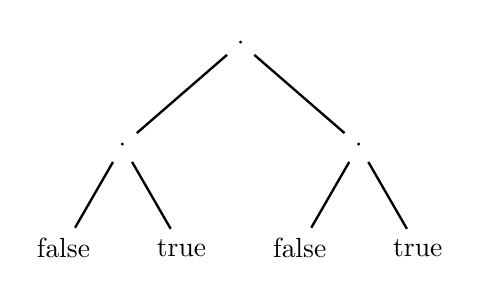
\begin{tikzpicture}[
    level 1/.style={sibling distance=30mm},
    level 2/.style={sibling distance=15mm}
  ]
    \node {$\cdot$}
      child{node {$\cdot$}
        child{node {\code{false}}}
        child{node {\code{true}}}
      }
      child{node {$\cdot$}
        child{node {\code{false}}}
        child{node {\code{true}}}
      }
    ;
  \end{tikzpicture}
\end{center}

which represents the set of bit strings $\{ 01, 11 \}$.

\newpage

\begin{parts}
  \part[5]\hfill

    Write a function \code{check} with the following specification:
    \spec
      {check}
      {\code{bdt -> bitstring -> bool}}
      {\code{bdt} is $n$-full, and \code{List.length bs} $\eeq$ \code{n}}
      {\code{check bdt bs} $\eeq$ \code{b}, where \code{b} is the contents of
      the \code{Final} node reached by reading the bits of \code{bs}.
      }

    \begin{solutionorbox}[15em]
      \begin{codeblock}
        fun check bdt bs =
          case (bdt, bs) of
            (Final b, []) => b
          | (Choice (l, r), Zero::bs) => check l bs
          | (Choice (l, r), One::bs) => check r bs
      \end{codeblock}
    \end{solutionorbox}

  \part[2]\hfill

    Write and solve a recurrence for the \textbf{work} of \code{check bdt},
    in terms of the length of the input list \code{bs},
    assuming valid inputs to \code{check} according to its precondition.

    \begin{solutionorbox}[20em]
      $W_{\code{check}}(0) = c_0$
      $W_{\code{check}}(n) = c_1 + W_{\code{check}}(n - 1)$

      So ultimately, $O(n)$.
    \end{solutionorbox}

  \newpage

  \part[5]\hfill

    We are also going to write a \code{partition} function, which we are going
    to need for later. This function will partition elements of a list according
    to some predicate function.
    True means left, false means right.

    For funsies, we will do it in CPS.

    Write a function with the following specification:
    \spec
      {partition}
      {\\ {\small\code{('a -> bool) -> 'a list -> ('a list * 'a list -> 'b) -> 'b}}}
      {\code{p} is total}
      {\code{partition p L k} $\eeq$ \code{k (A, B)} where
      \begin{itemize}
        \item for all \code{x} in \code{A}, \code{p x} $\eeq$ \code{true}
        \item for all \code{x} in \code{B}, \code{p x} $\eeq$ \code{false}
        \item \code{A @ B} contains the same elements as \code{L}
      \end{itemize}
      }

    such that \code{partition (fn x => x mod 2 = 0) [1, 2, 3] (fn x => x)}
    evaluates to \code{([2], [1, 3])}.

    \vspace{10pt}

    \textbf{Extra Credit:} For 2 extra points, instead write \code{partition} such
    that the predicate function \code{p} has type
    \code{'a -> ('a -> 'b) -> ('a -> 'b) -> 'b}.
    In other words, the predicate function itself takes in two continuations, where
    the first one is called on the input if the predicate function "likes" it,
    and the second one is called if the predicate function does not.

    \vspace{10pt}

    \begin{constraint}
      \code{partition} must be written in CPS.
    \end{constraint}

    \begin{solutionorbox}[20em]
      \begin{codeblock}
      fun partition p l sc =
        case l of
          [] => sc ([], [])
        | x::xs =>
          partition p xs (fn (l, r) =>
            if p x then
                sc (a :: l, r)
            else
                sc (l, b :: r)
          )

      (* extra credit! *)
      fun partition' p l sc =
        case l of
          [] => sc ([], [])
        | x::xs =>
          partition p l (fn (l, r) =>
            p x
              (fn a => sc (a :: l, r))
              (fn b => sc (l, b :: r))
          )
      \end{codeblock}
    \end{solutionorbox}

  \newpage

  \part[2]\hfill

    Now, write a function \code{partition_bstrs} to partition a list of bit
    strings into ones which start with \code{One} and ones which start with
    \code{Zero}.

    \spec
      {partition_bstrs}
      {\code{bitstring list -> (bitstring list * bitstring list -> 'a) -> 'a}}
      {\code{bstrs} is a list of non-empty bit strings}
      {\code{partition_bstrs bstrs k} $\eeq$ \code{k (L, R)} such that
        \code{L} contains all bit strings in \code{bstrs} starting with a 0, and
        \code{R} contains all bit strings in \code{bstrs} starting with a 1.
      }

    \vspace{10pt}

    \textbf{Extra Credit:} For 2 extra points, write \code{partition_bstrs} using the
    extra credit version of \code{partition}.

    \vspace{10pt}

    \begin{constraint}
      You may not use the \code{fun} keyword. You are allowed a single
      \code{fn} expression, unless you're doing the extra credit, in which
      case you're allowed 3.
    \end{constraint}

    \begin{solutionorbox}[20em]
      \begin{codeblock}
        val partition_bstrs =
          partition
            (fn Zero :: _ => true
              | One  :: _ => false
            )

        val partition_bstrs' =
          partition
            (fn cs => fn scl => fn scr =>
              case cs of
                Zero :: cs => scl (Zero :: cs)
              | One :: cs => scr (One :: cs)
              | _ => raise Precondition
            )
      \end{codeblock}
    \end{solutionorbox}

  \begin{EnvUplevel}
    However, checking can be a little redundant. Suppose that our set of
    bit strings is the set $\{ 00, 01, 10, 11 \}$. Then,
    we could do the work to query this set, or we could
    just observe that the answer is always \code{true}!

    This is because this set contains every single bit string of length
    2. In other words, as an $2$-full tree, our BDT looks like this:

    \begin{center}
      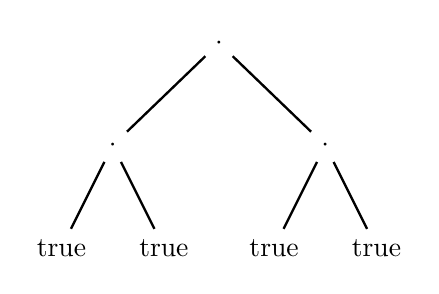
\begin{tikzpicture}[
        level 1/.style={sibling distance=27mm},
        level 2/.style={sibling distance=13mm}
      ]
        \node {$\cdot$}
          child{node {$\cdot$}
            child{node {\code{true}}}
            child{node {\code{true}}}
          }
          child{node {$\cdot$}
            child{node {\code{true}}}
            child{node {\code{true}}}
          }
        ;
      \end{tikzpicture}
    \end{center}

    but it may as well be described as the following tree:

    \vspace{10pt}

    \begin{center}
      \code{true}
    \end{center}

    \vspace{10pt}

    This is another way of saying that we can do some compression!

    \textbf{Definition.} A binary decision tree \code{bdt : bdt} is
    \textit{compressed} if the values \code{Choice (Final true, Final true)} and
    \code{Choice (Final false, Final false)} never appear in it anywhere.
  \end{EnvUplevel}



  \part[12]\hfill

    Now, let's get to the task of constructing our compressed BDT!

    Write a function \code{compress} with the specification:

    \spec
      {compress}
      {\code{int -> bitstring list -> bdt}}
      {\code{bstrs} is a list of unique bit strings, such that each bit string \code{bs} has
      that \code{List.length bs = n}}
      {\code{compress n bstrs} $\eeq$ the compressed BDT that
      represents the set of bit strings \code{bstrs}}

    \vspace{80pt}

    SPACE INTENTIONALLY LEFT BLANK -- KEEP READING

    \newpage

    I will use the shorthand of surrounding a bit string with curly braces to
    mean the corresponding SML value. For instance, \code{\{110\}} means
    \code{[One, One, Zero]}.

    Then, we should have that:
    \begin{itemize}
      \item \code{compress 1 []} $\eeq$ \code{Final false}, pictured by the BDT:

      \begin{center}
        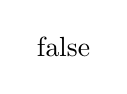
\begin{tikzpicture}[
          level distance=8mm,
          level 1/.style={sibling distance=50mm},
          level 2/.style={sibling distance=30mm},
          level 3/.style={sibling distance=15mm}
        ]
          \node {\code{false}}
          ;
        \end{tikzpicture}
      \end{center}
      \vspace{5pt}
      \item \code{compress 1 [\{0\}, \{1\}]} $\eeq$ \code{Final true}, pictured by the BDT:

      \begin{center}
        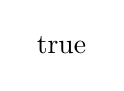
\begin{tikzpicture}[
          level distance=8mm,
          level 1/.style={sibling distance=50mm},
          level 2/.style={sibling distance=30mm},
          level 3/.style={sibling distance=15mm}
        ]
          \node {\code{true}}
          ;
        \end{tikzpicture}
      \end{center}
      \vspace{5pt}
      \item \code{compress 1 [\{0\}]} $\eeq$ \code{Choice (Final true, Final false)}, pictured by the BDT:

      \begin{center}
        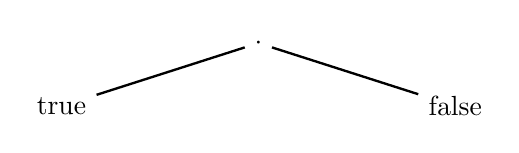
\begin{tikzpicture}[
          level distance=8mm,
          level 1/.style={sibling distance=50mm},
          level 2/.style={sibling distance=30mm},
          level 3/.style={sibling distance=15mm}
        ]
          \node {$\cdot$}
            child{node{\code{true}}}
            child{node{\code{false}}}
          ;
        \end{tikzpicture}
      \end{center}
      \vspace{5pt}
      \item \code{compress 1 [\{1\}]} $\eeq$ \code{Choice (Final false, Final true)}, pictured by the BDT:

      \begin{center}
        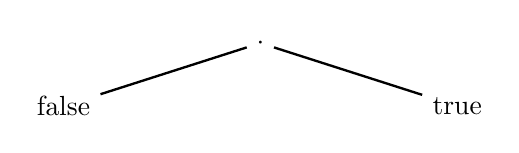
\begin{tikzpicture}[
          level distance=8mm,
          level 1/.style={sibling distance=50mm},
          level 2/.style={sibling distance=30mm},
          level 3/.style={sibling distance=15mm}
        ]
          \node {$\cdot$}
            child{node{\code{false}}}
            child{node{\code{true}}}
          ;
        \end{tikzpicture}
      \end{center}
      \vspace{5pt}
      \item \code{compress 2 [\{00\}, \{01\}, \{10\}, \{11\}]} $\eeq$ \code{Final true}, pictured by the BDT:

      \begin{center}
        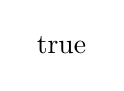
\begin{tikzpicture}[
          level distance=8mm,
          level 1/.style={sibling distance=50mm},
          level 2/.style={sibling distance=30mm},
          level 3/.style={sibling distance=15mm}
        ]
          \node {\code{true}}
          ;
        \end{tikzpicture}
      \end{center}
      \vspace{5pt}
      \item \code{compress 3 [\{000\}, \{110\}, \{101\}, \{100\}]} $\eeq$
      \begin{codeblock}
        Choice
          ( Choice
              (Choice (Final true, Final false), Final false),
            Choice
              (Final true, Choice (Final true, Final false))
          )
      \end{codeblock}
    \end{itemize}
    which denotes the BDT of
    \begin{center}
      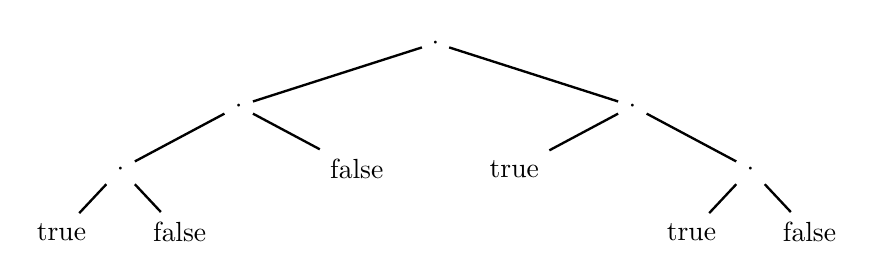
\begin{tikzpicture}[
        level distance=8mm,
        level 1/.style={sibling distance=50mm},
        level 2/.style={sibling distance=30mm},
        level 3/.style={sibling distance=15mm}
      ]
        \node {$\cdot$}
          child{node {$\cdot$}
            child{node {$\cdot$}
              child{node {\code{true}}}
              child{node {\code{false}}}
            }
            child{node {\code{false}}}
          }
          child{node {$\cdot$}
            child{node {\code{true}}}
            child{node {$\cdot$}
              child{node {\code{true}}}
              child{node {\code{false}}}
            }
          }
        ;
      \end{tikzpicture}
    \end{center}

    \newpage

    Reproduced for your convenience: write a function \code{compress} with the
    specification:

    \spec
      {compress}
      {\code{int -> bitstring list -> bdt}}
      {\code{bstrs} is a list of unique bit strings, such that each bit string \code{bs} has
      that \code{List.length bs = n}}
      {\code{compress n bstrs} $\eeq$ the compressed BDT that
      represents the set of bit strings \code{bstrs}}

    You may assume that you are given \code{pow : int * int -> int}, such that
    \code{pow (n, k)} $\eeq$ $n^k$, and \code{tl : 'a list -> 'a list}, which
    obtains the rest of a list after the first element (if possible), and raises an exception otherwise.

    \textbf{Hint:} A reasonably simple solution uss \code{pow}, \code{tl}, and
    \code{partition_bstrs}.

    \textbf{Hint 2:} There are $2^n$ bit strings of length $n$.

    If your solution looks convoluted, you're probably overthinking it.

    \begin{solutionorbox}[30em]
      \begin{codeblock}
        fun compress (n : int) (bstrs : bitstring list) =
          if List.length bstrs = pow (2, n) then
            (* must be full *)
            Final true
          else if List.length bstrs = 0 then
            Final false
          else
            partition_bstrs bstrs (fn (l, r) =>
              Choice
                ( compress (n - 1) (List.map tl l)
                , compress (n - 1) (List.map tl r)
                )
            )
      \end{codeblock}
    \end{solutionorbox}

  \newpage

  \part[2]\hfill

    Consider the specification of \code{check}, which has been reproduced
    for your convenience here:
    \spec
      {check}
      {\code{bdt -> bitstring -> bool}}
      {\code{bdt} is $n$-full, and \code{List.length bs} $\eeq$ \code{n}}
      {\code{check bdt bs} $\eeq$ \code{b}, where \code{b} is the contents of
      the \code{Final} node reached by reading the bits of \code{bs}.
      }

    When checking compressed BDTs, this specification does not quite match.

    Write a new \code{REQUIRES} clause for \code{check} to make it compatible
    with compressed BDTs.

    \begin{solutionorbox}[6em]
      \code{bdt} is a compressed BDT, and \code{List.length bs} $\eeq$ \code{n}
    \end{solutionorbox}

  % \part[5]\hfill

  %   Write and solve a recurrence which denotes the \textbf{work} of \code{compress},
  %   in terms of the input value \code{n}, assuming that preconditions hold.

  %   % state the work of pow and partition_strs

  %   Show your work.

  %   \begin{solutionorbox}[19em]
  %     $W_{\code{compress}}(0) = c_0$
  %     $W_{\code{compress}}(n) = O(2^n) + 2 \cdot W_{\code{compress}}(n - 1)$

  %     \begin{align*}
  %       W_{\code{compress}}(n) \\
  %       &= O(2^n) + 2 \cdot W_{\code{compress}}(n - 1) \\
  %       &= O(2^n) + 2 \cdot (O(2^{n - 1}) + W_{\code{compress}}(n - 2)) \\
  %       &= O(2^n) + O(2^n) + W_{\code{compress}}(n - 2)
  %     \end{align*}

  %     This evaluates to $\Sum_{i = 0}^n O(2^n) = O(n2^n)$.
  %   \end{solutionorbox}

  % \part[5]\hfill

  %   Write and solve a recurrence which denotes the \textbf{span} of \code{compress},
  %   in terms of the input value \code{n}, assuming that preconditions hold.

  %   Assume that \code{partition_strs} partitions approximately evenly, and runs in
  %   linear time in its input list length.

  %   Show your work.

  %   \begin{solutionorbox}[19em]
  %     $S_{\code{compress}}(0) = c_0$
  %     $S_{\code{compress}}(n) = O(2^n) + S_{\code{compress}}(n - 1)$

  %     \begin{align*}
  %       S_{\code{compress}}(n) \\
  %       &= O(2^n) + \cdot S_{\code{compress}}(n - 1) \\
  %       &= O(2^n) + O(2^{n - 1}) + S_{\code{compress}}(n - 2)
  %     \end{align*}

  %     This evaluates to $1 + 2 + ... + 2^n = O(2^n)$.
  %   \end{solutionorbox}

  % \newpage

  % \part[10]\hfill

  %   Write a function \code{insert} which satisfies the following
  %   specification:
  %   \spec
  %     {insert}
  %     {\code{bdt -> char list -> bdt}}
  %     {\code{bt} is a compressed BDT and \code{cs} is a bit string that cannot
  %     be shorter than any bit string in \code{bt}}
  %     {\code{insert bt cs} evaluates to the BDT which now contains
  %     the bit string \code{cs}, but is otherwise equivalently compressed}

  %   \begin{solutionorbox}[30em]
  %     \begin{codeblock}
  %       fun insert (bt : bdt) (cs : char list) =
  %         case (bt, cs) of
  %           (_, []) => Final true
  %         | (Choice (L, R), #"0"::cs') =>
  %             Choice (insert L cs', R)
  %         | (Choice (L, R), #"1"::cs') =>
  %             Choice (L, insert R cs')
  %         | (Final b, #"0"::cs') =>
  %             Choice (insert L cs', Final b)
  %         | (Final b, #"1"::cs') =>
  %             Choice (Final b, insert R cs')
  %         | _ => raise Precondition
  %     \end{codeblock}
  %   \end{solutionorbox}

  \part[5]\hfill

    Now, we can compress our bit string sets, and query them.

    Consider the following such function:

    \begin{codeblock}
      fun query (n : int) (bstrs : bitstring list) (bs : bitstring) =
        check (compress n bstrs) bs
    \end{codeblock}

    Suppose we are interested in repeat queries to the same set of bit strings.
    There is an inefficiency in this code. Rewrite \code{query} to perform better
    in that case.

    \begin{solutionorbox}[15em]
      \begin{codeblock}
        fun query (n : int) (bstrs : bitstring list) =
          let
            val bdt = compress n bstrs
          in
            fn bs => check bdt bs
          end
      \end{codeblock}
    \end{solutionorbox}
\end{parts}

\newpage
\titledquestion{Level Order Traversal}

\textbf{Level Order Traversal}

Recall the problem of \textit{tree traversal}, which is the problem of visiting
the elements of a tree in some prescribed order.

We have discussed several tree traversals, such as \textit{postorder},
\textit{inorder}, and \textit{preorder}, which are classic recursive traversals.
Less straightforward is what is known as a \textit{level-order traversal}, which
traverses a tree in the same way that a human would read a book.

\begin{center}
  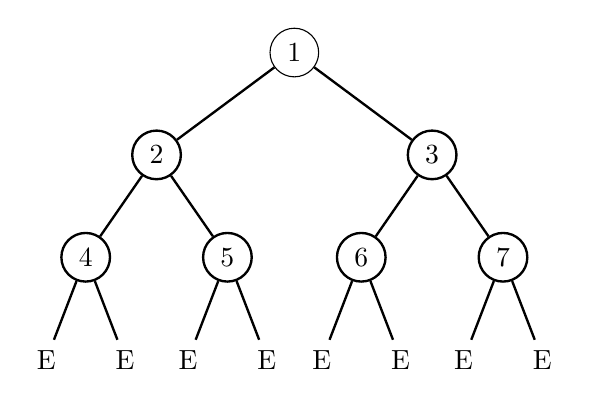
\begin{tikzpicture}[
          level 1/.style={sibling distance=35mm},
          level 2/.style={sibling distance=18mm},
          level 3/.style={sibling distance=10mm},
          level distance=13mm,
          circ/.style={draw=black, circle}
        ]
    \node[circ] {1}
      child{node[circ] {2}
        child{node[circ] {4}
          child{node {\code{E}}}
          child{node {\code{E}}}
        }
        child{node[circ] {5}
          child{node {\code{E}}}
          child{node {\code{E}}}
        }
      }
      child{node[circ] {3}
        child{node[circ] {6}
          child{node {\code{E}}}
          child{node {\code{E}}}
        }
        child{node[circ] {7}
          child{node {\code{E}}}
          child{node {\code{E}}}
        }
      }
    ;

  \end{tikzpicture}
\end{center}

This is quite difficult to implement, recursively, via naively computing
the level order traversal of children. However, by changing our perspective,
it turns out we can actually still solve this recursively.

We will do this by writing the following helper:
\spec
  {levelord}
  {\code{'a tree -> 'a list stream}}
  {\code{true}}
  {\code{levelord T} evaluates to the stream \code{S}, such that the
  $i$th element of \code{S} contains all of the elements in the $i$th
  level of the tree \code{T}.}

So for instance, if \code{T} is the above tree, we should have that:
\begin{itemize}
  \item \code{levelord T} $\eeq$ \code{Stream.fromList [[1],[2, 3],[4, 5, 6, 7],[]]}
  \item \code{levelord Empty} $\eeq$ \code{Stream.fromList [[]]}
  \item \code{levelord (N(E,1,E))} $\eeq$ \code{Stream.fromList [[1], []]}
  \item \code{levelord (N(N(E,2,E),1,E))} $\eeq$ \code{Stream.fromList [[1], [2], []]}
\end{itemize}

(The empty lists are because the corresponding level of the tree still has stuff
in it, it's just all \code{Empty}s)

\newpage

We will also give you this helper function, which you will need:

\spec
  {zipAppend}
  {{\small\code{'a list stream -> 'a list stream -> 'a list stream}}}
  {\code{true}}
  {\code{zipAppend S1 S2} evaluates to the stream which pairs up elements from
  \code{S1} and \code{S2}, appending their corresponding lists. If one doesn't
  exist in one of the streams, it simply takes the other list.}

\begin{codeblock}
  fun zipAppend S1 S2 =
    case (S.expose S1, S.expose S2) of
      (S.Empty, _) => S2
    | (_, S.Empty) => S1
    | (S.Cons (x, S1'), S.Cons (y, S2')) =>
        S.cons (x @ y, zip S1' S2')
\end{codeblock}

\begin{parts}
  \part[2]\hfill
    Is \code{zipAppend} maximally lazy? If not, explain why, and how it may be fixed.

    \begin{solutionorbox}[8em]
      No, because it exposes the streams before an element is requested.
      You should instead write:

      \begin{codeblock}
        fun zipAppend S1 S2 =
          S.delay (fn () =>
            case (S.expose S1, S.expose S2) of
              (S.Empty, _) => S2
            | (_, S.Empty) => S1
            | (S.Cons (x, S1'), S.Cons (y, S2')) =>
                S.cons (x @ y, zip S1' S2')
          )
      \end{codeblock}
    \end{solutionorbox}
  \part[8]\hfill

    Implement \code{levelord} as described above.

    \textbf{Hint:} This problem is about reasoning via specification. Do not get
    lost in the nitty gritty. Think recursively.

    This problem can be solved in three lines.

    \begin{solutionorbox}[12em]
      \begin{codeblock}
        fun levelord Empty = S.cons ([], S.empty)
          | levelord (Node (L, x, R)) =
              S.cons ([x], (zipAppend (levelord L) (levelord R)))
      \end{codeblock}
    \end{solutionorbox}

  \newpage

  \part[5]\hfill

    Let's now implement a function which will take us back from
    \code{'a list stream} to \code{'a list}.

    \spec
      {flatten'}
      {\code{'a list stream -> 'a list}}
      {\code{S} is productive and finite}
      {\code{flatten' S} $\eeq$ \code{flatten (Stream.toList S)}}

    \begin{constraint}
      You cannot use \code{Stream.toList}.
    \end{constraint}

    \begin{solutionorbox}[15em]
      \begin{codeblock}
        fun flatten' S =
          case S.expose S of
            Empty => []
          | Cons (x, S') => x @ flatten' S'
      \end{codeblock}
    \end{solutionorbox}

  \part[2]\hfill

    Implement \code{levelord' : 'a tree -> 'a list}, finally, in terms of
    the functions that we have used previously.

    \begin{constraint}
      You may not use any \code{fun} declarations or \code{fn} expressions.
    \end{constraint}

    \begin{solutionorbox}[8em]
      \begin{codeblock}
        val levelord' = flatten' o levelord
      \end{codeblock}
    \end{solutionorbox}
\end{parts}

\newpage
\titledquestion{File Systems}

\textbf{File Systems}

Consider the structure of a Linux file system, which is composed of \textit{directories}
and \textit{files}.

A directory is a structure which may contain further directories and files. A file
is just a standalone piece of data.

We may represent it via the following SML type:\footnote{Which is (almost) isomorphic to
a \code{string rose}, for those of you keeping track at home.}
\begin{codeblock}
  datatype filesys =
      File of string
    | Dir of string * filesys list

  type filesys = (string * data) list
  and data = File | Dir of filesys
\end{codeblock}

A \textit{file system} is a value of type \code{filesys} such that for each
\code{Dir (d, ds)}, no \code{File} or \code{Dir} in \code{ds} shares the
same name.

So for instance, a file system with the following structure:

\begin{minipage}{\linewidth} % Use a minipage to control the width
  \dirtree{%
  .1 root.
  .2 A.
  .3 foo.sml.
  .3 bar.txt.
  .2 B.
  .3 baz.sml.
  .2 C.
  }
\end{minipage}

would be represented by the following SML value:
\begin{codeblock}
  Dir ("root",
    [ Dir ("A", [ File "foo.sml", File "bar.txt" ]),
      Dir ("B", [ File "baz.sml"]),
      Dir ("C", [])
    ]
  )
\end{codeblock}

\newpage

You are given an implementation of the \code{cd} function, which allows
moving through the file system, according to the following specification:

\spec
  {cd}
  {\code{filesys -> string list -> filesys option}}
  {\code{true}}
  {\code{cd fs path} takes the moves indicated by the path \code{path},
  and returns \code{SOME fs'} if that ends up at a file system,
  and \code{NONE} if it doesn't.}

So for the above filesystem, if it was to be bound to \code{fs}, we would
have that:
\begin{itemize}
  \item \code{cd fs []} $\eeq$ \code{SOME fs}
  \item \code{cd fs ["B"]} $\eeq$ \code{SOME (Dir ("B", [ File "baz.sml" ]))}
  \item \code{cd fs ["root"]} $\eeq$ \code{NONE}
\end{itemize}

The given implementation is:

\begin{codeblock}
  fun cd fs [] = fs
    | cd (File _) (s::rest) = NONE
    | cd (Dir (dir, ds)) (s::rest) =
        List.foldl
          (fn (_, SOME res) => SOME res
            | (File _, _) => NONE
            | (Dir (dir', ds'), _) =>
                if s = dir' then
                  cd (Dir (dir', ds')) rest
                else
                  NONE
          )
          NONE
          ds
\end{codeblock}

\begin{parts}
  \part[6]\hfill

    Assume that any directory in a given file system has $k$
    many entries in it, and it is roughly balanced.

    Write and solve a recurrence for the \textbf{work} of \code{cd} on
    such a file system, in terms of the \textbf{depth} of the file system.
    The depth of a file system is, intuitively, the maximum number of
    nested directories you can go into.

    \begin{solutionorbox}[18em]
      $W_{\code{cd}}(0) = c_0$
      $W_{\code{cd}}(d) = O(k) + W_{\code{cd}}(d - 1)$

      So ultimately, $O(kd)$.
    \end{solutionorbox}

    \begin{EnvUplevel}
      Consider the following function on file systems:

      \begin{codeblock}
        fun countdirs (File _) = 0
          | countdirs (Dir (_, dirs)) =
              List.map countfiles dirs
              |> List.foldl (op+) 1
      \end{codeblock}
    \end{EnvUplevel}

  \part[5]\hfill

    Assume that any directory in a given file system has $k$
    many entries in it, and it is roughly balanced.

    Write but \textbf{do not solve} a recurrence for the \textbf{work} of
    \code{countdirs} on such a file system, in terms of the \textbf{nodes} of
    the file system. The nodes of a file system is, intuitively, the total
    number of files and directories in it.

    \begin{solutionorbox}[18em]
      $W_{\code{cd}}(0) = c_0$
      $W_{\code{cd}}(n) = O(k) + k \cdot W_{\code{cd}}(n / k)$
    \end{solutionorbox}

  \newpage

  \part[6]\hfill

    Assume that any directory in a given file system has $k$
    many entries in it, and it is roughly balanced.

    Write and solve a recurrence for the \textbf{span} of \code{countdirs} on
    such a file system, in terms of the \textbf{nodes} of the file system.
    The nodes of a file system is, intuitively, the total number of
    files and directories in it.

    \textbf{For this problem, and only this problem, pretend that \code{List.map}
    runs each call in parallel.}

    \begin{solutionorbox}[20em]
      $S_{\code{cd}}(0) = c_0$
      $S_{\code{cd}}(n) = O(k) + S_{\code{cd}}(n / k)$

      So ultimately, $O(k \cdot \log_k n)$.
    \end{solutionorbox}





  % \part[5]\hfill

  %   Assume that any directory in a given file system has, at maximum, $k$
  %   many entries in it.

  %   Write a recurrence for the \textbf{span} of \code{cd} on
  %   such a file system, in terms of the \textbf{depth} of the file system.
  %   The depth of the file system is, intuitively, the maximum number of
  %   nested directories you can go into.

  %   You may find useful the fact that $1 + k + k^2 + ... + k^n$ is on the order
  %   of $O(k^n)$, for non-zero $k$.

  %   \begin{solutionorbox}[8em]
  %     $S_{\code{cd}}(0) = c_0$
  %     $S_{\code{cd}}(d) = O(k) + \cdot S_{\code{cd}}(d - 1)$
  %   \end{solutionorbox}


  \newpage

  \part[10]\hfill

    Implement \code{absolutize}, which replaces all of the names in the file
    system with its absolute path. (which should start with a "/"). For
    instance, running \code{absolutize} on the above example file system should
    give you
    \begin{codeblock}
      Dir ("/root",
        [ Dir ("/root/A", [ File "/root/A/foo.sml",
                            File "/root/A/bar.txt" ]),
          Dir ("/root/B", [ File "/root/B/baz.sml"]),
          Dir ("/root/C", [])
        ]
      )
    \end{codeblock}

    \spec
      {absolutize}
      {\code{filesys -> filesys}}
      {\code{true}}
      {\code{absolutize fs} replaces each file and directory's name with
      the absolute path required to get there}

    \begin{solutionorbox}[30em]
      \begin{codeblock}
        fun mkPath strs =
          List.foldl (fn (x, acc) =>
            acc ^ "/" ^ x
          ) "" strs

        fun absolutize' cur (File s) = File (mkPath (s :: cur))
          | absolutize' cur (Dir (dir, ds)) =
              let
                val new_cur = dir :: cur
              in
                Dir (mkPath new_cur, List.map (absolutize new_cur) ds)
              end

        fun absolutize = absolutize' []
      \end{codeblock}
    \end{solutionorbox}
\end{parts}

\newpage
\titledquestion{Extra Credit: Type Design}

\textbf{Extra Credit: Type Design}

Consider the problem of animals on a farm.

You have cats, dogs, horses, and cows. They have the following specifications:
\begin{itemize}
  \item All of the animals have names.
  \item Some cows were bought from other farmers, meaning that they
  have an associated name of their seller, and a price (which is a \code{real})
  that they were bought for. All other animals were raised on the farm, though.
  \item All dogs have a working status, which is either primarily as a pet,
  a herder, or a guard dog. If the dog is a pet, then it also has a best friend,
  who has a name. All other animals are unemployed.
  \item The horses all have a particular day of the week that they prefer to
  run on. Some of them have two.
  \item Some horses are champion racehorses, and have any number of named accolades
  that they personally have won. We are interested in the names of those accolades,
  specifically.
  \item None of the animals are particularly big fans of Smash Mouth.
\end{itemize}

\vspace{20pt}

\begin{center}
\includegraphics{farms.png}
\end{center}

\newpage

\begin{parts}
  \bonuspart[5]\hfill

    Come up with a type \code{animal} that faithfully represents the information
    of an animal on the farm. This type should have no illegal representation,
    meaning that any value of this type should represent all and only
    the relevant information to one of those specific animals.

    It should also be as un-redundant as possible, meaning there should not be
    different values that represent the same animal. It should also be as
    simple and elegant as possible.

    You may use as many \code{type} and \code{datatype} declarations as you wish.

    \begin{solutionorbox}[35em]
      \begin{codeblock}
        datatype dog_job = Pet of string | Herder | Guard

        datatype day = M | Tu | We | Th | F | Sa | Su

        type seller_info = string * real

        datatype animal_kind =
            Dog of dog_job
          | Cat
          | Horse of day * day option * string list
          | Cow of seller_info option

        type animal = string * animal_kind
      \end{codeblock}
    \end{solutionorbox}
\end{parts}

\newpage

\textbf{Appendix: The \code{SEQUENCE} Signature}

\begin{codeblock}
  signature SEQUENCE =
    sig
      (* ... *)

      val empty : unit -> 'a seq
      val singleton : 'a -> 'a seq
      val tabulate : (int -> 'a ) -> int -> 'a seq
      val fromList : 'a list -> 'a seq

      val nth : 'a seq -> int -> 'a
      val null : 'a seq -> bool
      val length : 'a seq -> int
      val toList : 'a seq -> 'a list

      val filter : ('a -> bool) -> 'a seq -> 'a seq
      val map : ('a -> 'b) -> 'a seq -> 'b seq
      val reduce : ('a * 'a -> 'a) -> 'a -> 'a seq -> 'a

      (* ... *)
    end
\end{codeblock}

\vspace{20pt}

\textbf{Appendix: The \code{STREAM} Signature}

\begin{codeblock}
signature STREAM =
  sig
    (* ... *)

    val delay : (unit -> 'a front) -> 'a stream
    val expose : 'a stream -> 'a front

    val empty : 'a stream
    val cons : 'a * 'a stream -> 'a stream
    val fromList : 'a list -> 'a stream
    val tabulate : (int -> 'a) -> 'a stream

    (* ... *)
  end
\end{codeblock}



% ------------------------------------------------------------------------------

\end{document}